\subsubsection{Design of Instruction Set} \label{sec:design-instruction-set}

OlaVM uses the Reduced Instruction Set Computer (RISC) architecture, one of its main features is a small instruction set, as opposed
to the Complex Instruction Set Computer(CISC) architecture.The difference between the two can be found in
\href{https://cs.stanford.edu/people/eroberts/courses/soco/projects/risc/risccisc/}{RISC vs. CISC}.

\emph{1. A reduced instruction set reduces the number of constraint polynomials}

In ZKVM, there is a very critical constraint, the CSTC (CPU State Transition Constraint); it is mainly used to constrain the validity
of VM state changes before and after the execution of an instruction.

\begin{figure}[!ht]
    \centering
    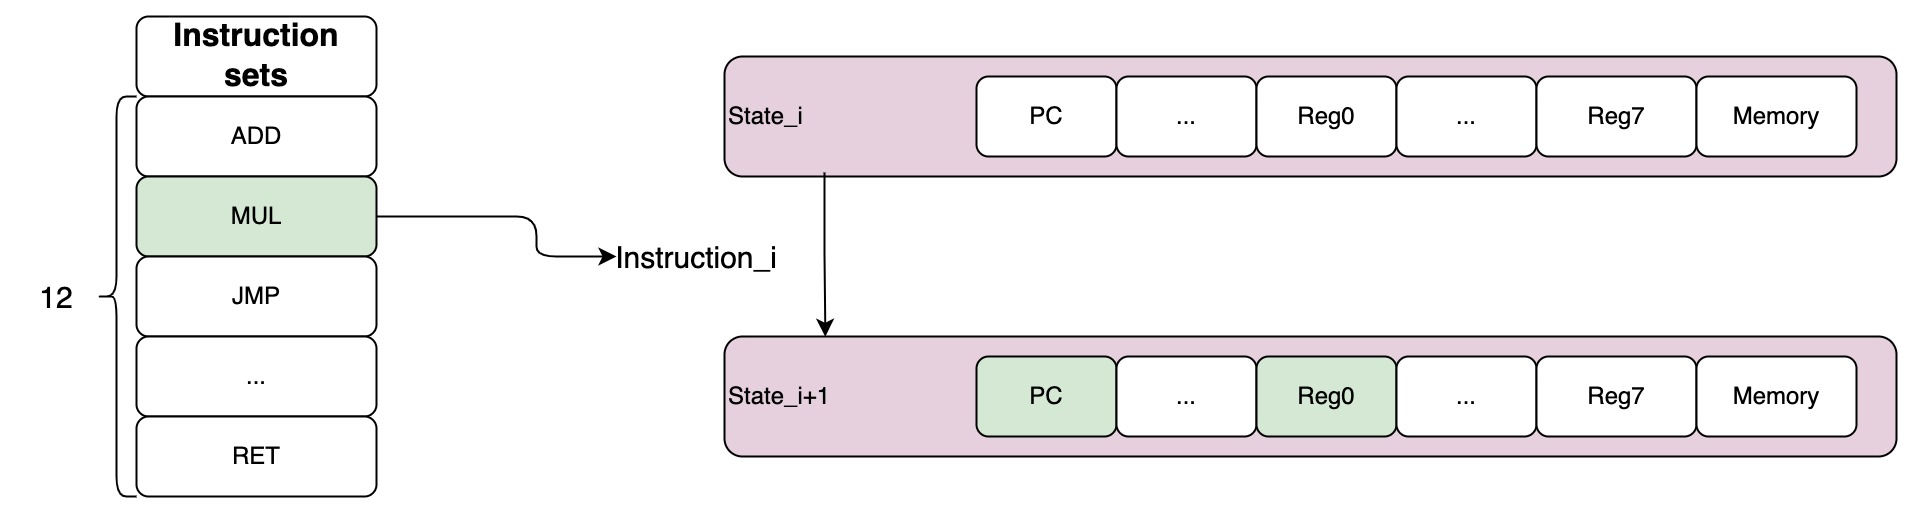
\includegraphics[width=0.8\textwidth]{vm/olavm-instruction-state.jpeg}
    \caption{Instruction-induced cpu state transition}
    \label{fig:instruction-cpu-state-transition}
\end{figure}

As shown in \figref{fig:instruction-cpu-state-transition}, there are many registers in the VM. When VM executes an instruction, it will
cause the state of some registers to change, so to ensure the correctness of VM execution, we need to constrain:
\begin{itemize}
    \item The change of register state involved in the execution of the instruction is valid;
    \item The status of registers not involved in the instruction execution remains unchanged.
\end{itemize}

Let's look at a simple example to explain the constraints on register state changes:
\begin{table}[!ht]
    \centering
    \begin{tabular}{|c|c|c|c|c|c|c|c|}
        \hline
        \rowcolor{gray} clk & pc    & instruction        & \dots & reg0  & reg1  & reg2  & \dots \\
        \hline
        \dots               & \dots & \dots              & \dots & \dots & \dots & \dots & \dots \\
        \hline
        78                  & 8     & ADD reg0 reg0 reg1 & \dots & 1     & 2     & 0     & \dots \\
        \hline
        79                  & 9     & MOV reg2 3         & \dots & 3     & 0     & 0     & \dots \\
        \hline
        80                  & 11    & JMP 2              & \dots & 3     & 0     & 3     & \dots \\
        \hline
        81                  & 2     & \dots              & ...   & 3     & 0     & 3     & \dots \\
        \hline
    \end{tabular}
    \caption{Example of cpu state transitions}
    \label{table:example-cpu-state-transitions}
\end{table}

Table \ref{table:example-cpu-state-transitions} briefly presents the changes of some registers after the VM executes three
instructions;taking the PC register as an example, the logic of the updates of the three instructions are:
\begin{itemize}
    \item ADD: $\mathrm{pc}_{i+1} = \mathrm{pc}_i + 1$
    \item MOV: $\mathrm{pc}_{i+1} = \mathrm{pc}_i + 2$
    \item JMP: $\mathrm{pc}_{i+1} = 2$
\end{itemize}

From the point of view of constraints, we do not know which instruction the VM is going to execute each time, so we have to
design a constraint that can handle all instructions, which we call (CSTC) CPU State Transition Constraint.For the simple
example above, we can design the update logic of the PC as follows:
\[ \mathrm{pc}_{i+1} = \mathrm{sel\_jmp}_i \cdot \mathrm{imm_value} + (1 - \mathrm{sel\_jmp}) \cdot (\mathrm{pc}_i + 1 + \mathrm{op1_imm}) \]

We write all state transitions of the cpu in this constrained form.The addition of each instruction adds new selectors resulting
in increased constraint complexity, so we limit the size of instructions to 19 (including builtins).

Of course, even though we have a lean instruction set architecture, we still need to maintain the Turing-complete feature so that
we can still compute everything based on these simple instruction sets.So that based on these simple instruction sets, we can still
compute everything that can be computed.Based on these instructions, combined with the prophet mechanism, we build a Turing-complete
DSL, O-lang, that supports loops and recursive operations.

\emph{2. Most of the operations will use a small part of the instruction set}

Under the CISC architecture, a large instruction set is defined.However, in reality, each instruction is used differently and for most
of the computations, only a small part of the instruction set may be used.From the constraint point of view, this is a big waste because
the constraint logic of all instructions needs to be included in the constraint system (CSTC), and the worst case would be that each instruction
would correspond to a constraint factor, thus making the whole constraint scale complex, including the number of polynomials and the order of
the constraints.

\begin{figure}[!ht]
    \centering
    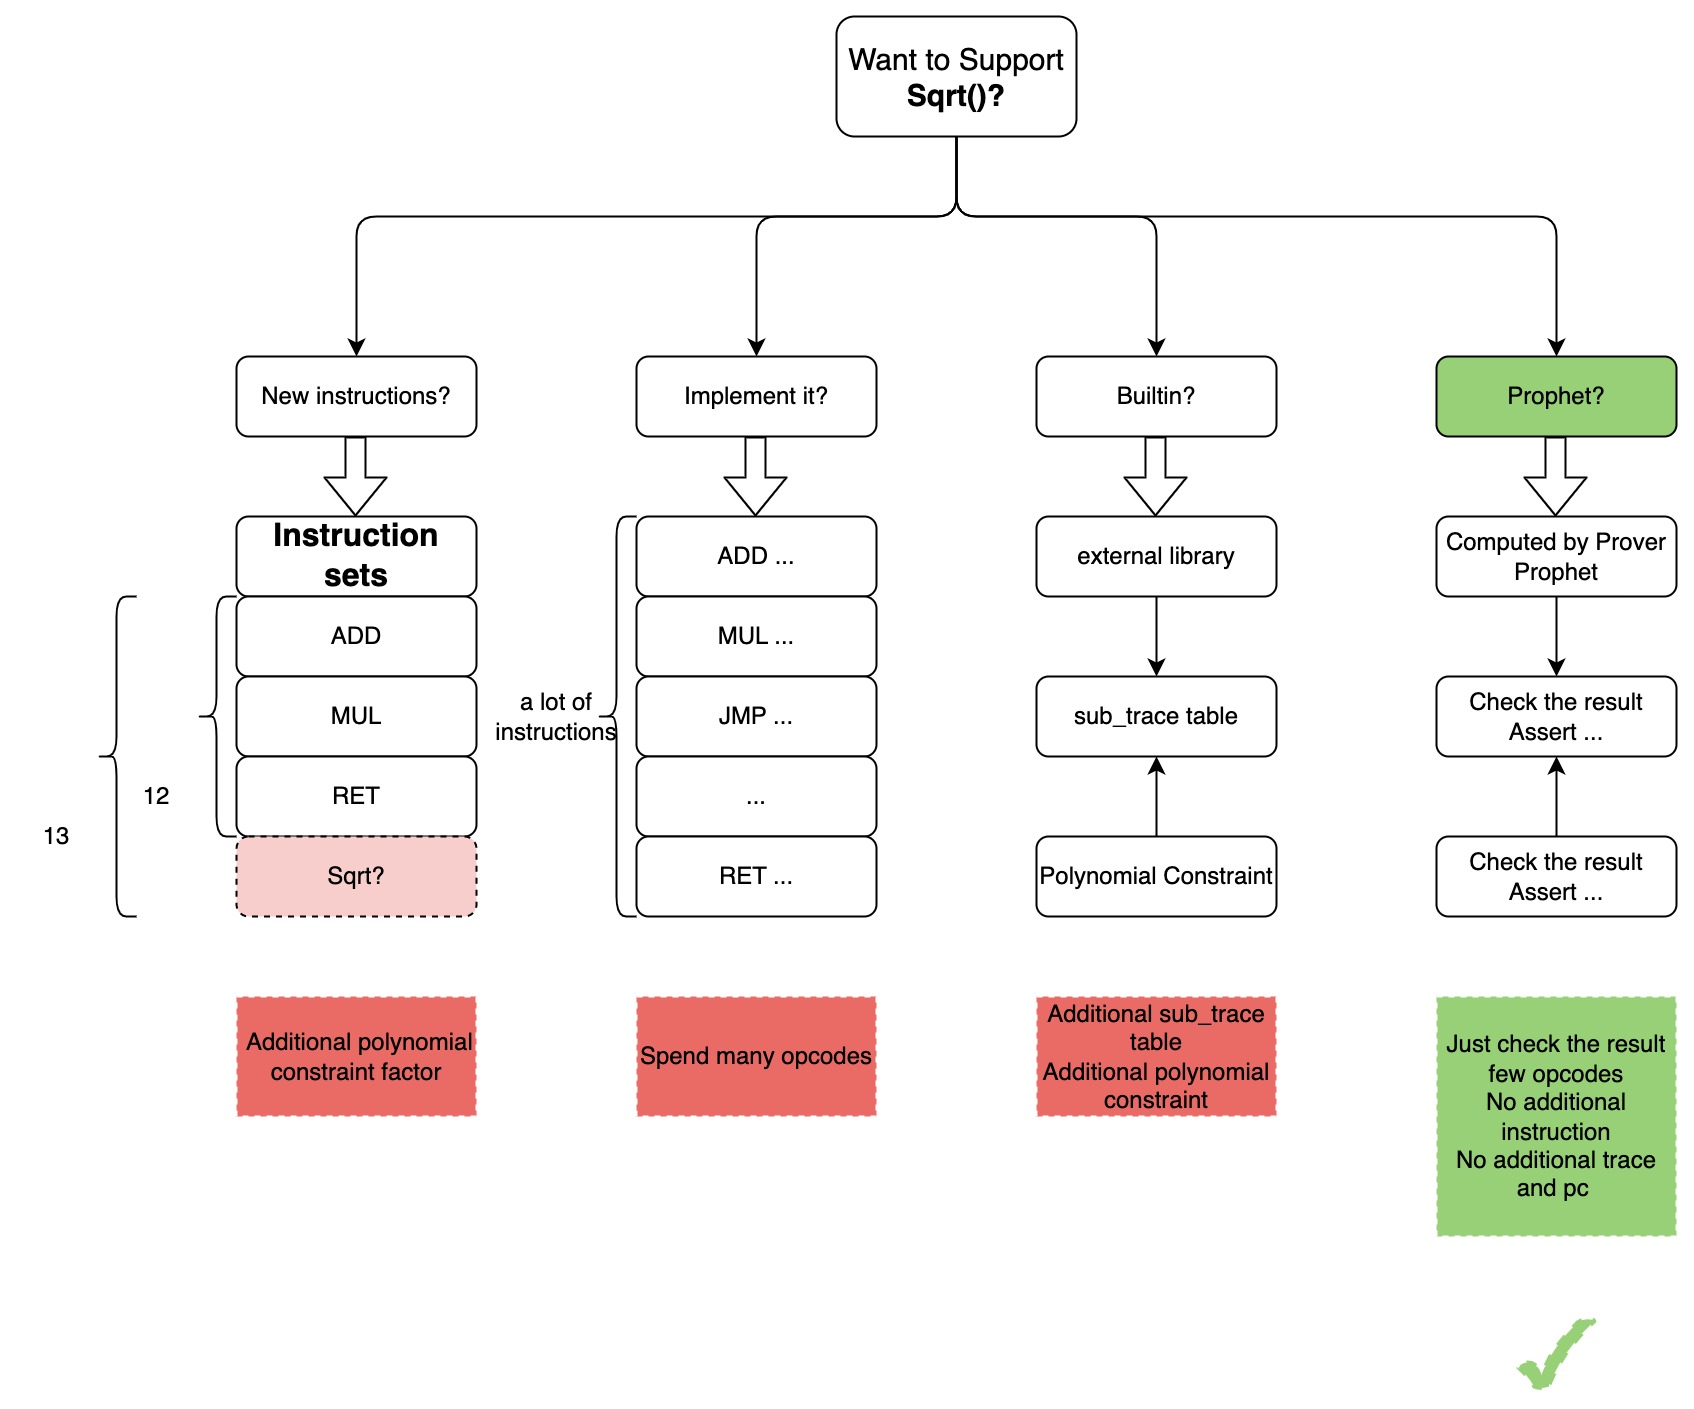
\includegraphics[width=0.8\textwidth]{vm/design-support-zk-unfriendly.jpeg}
    \caption{The best way to support ZK-Unfriendly computation}
    \label{fig:desgin-support-zk-unfriendly}
\end{figure}

If we are a reduced instruction set and Turing-complete, it is better to implement it with the existing instruction set than to introduce a new
instruction;although this will make the program bigger (more opcode), some redundant data will be added during the verification itself to
facilitate doing the FFT; but if it is a complex computation that requires a particularly large number of instructions to implement, we still
have ways to solve it, such as introducing Builtins and Prophet, whose principles we will focus on in later chapters, where you just need to
know that they can help drastically reduce the consumption of instructions to implement these complex computations, as shown in \figref{fig:desgin-support-zk-unfriendly}.